\begin{figure}
  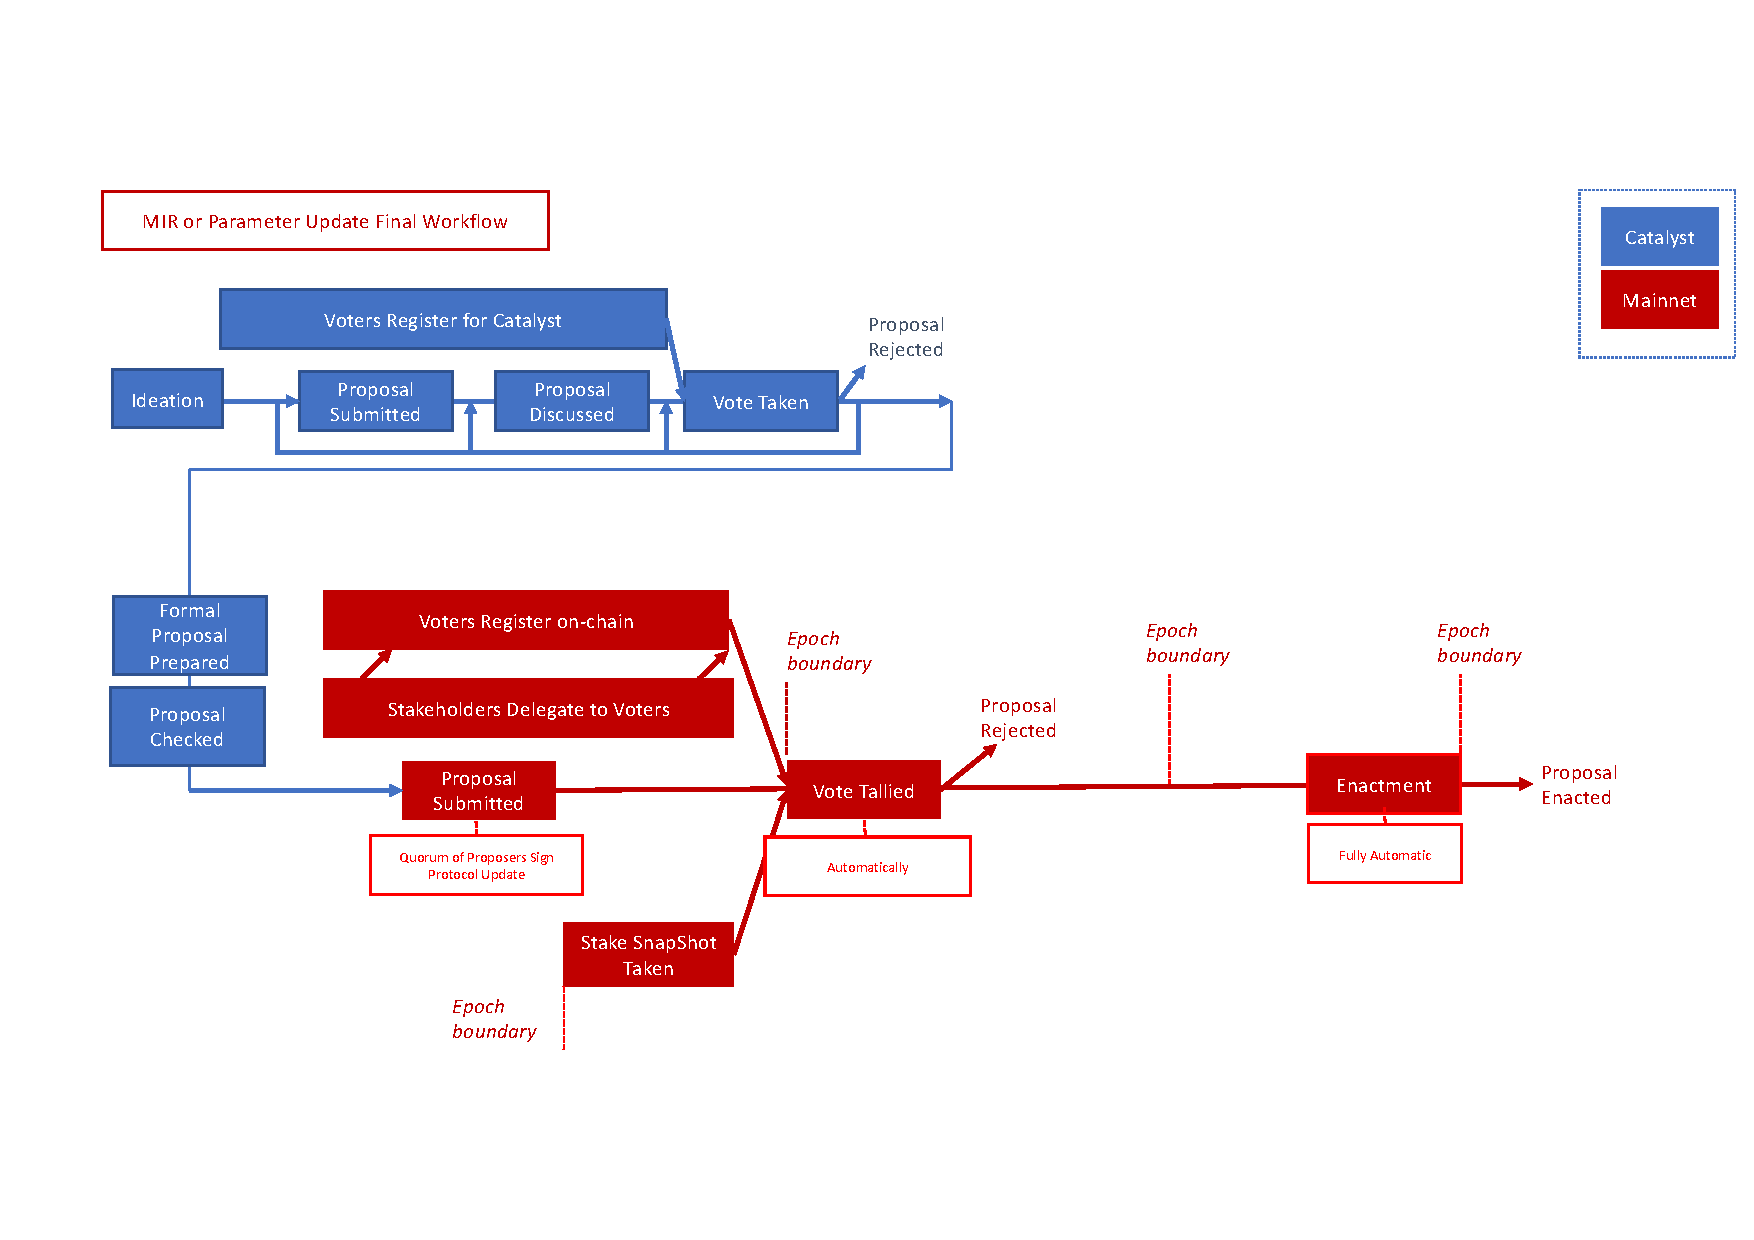
\includegraphics[trim=0 90 0 80,clip,width=\textwidth]{Workflow3}
  \caption{Example Workflow: Funds Transfer (MIR) or Simple Parameter Value Update}
  \label{fig:workflow-mir}
\end{figure}

\section{Example Workflows}
\label{sec:workflows}

Figures~\ref{fig:workflow-mir}-\ref{fig:workflow-hf} show outline workflows for
typical use cases.  Figure~\ref{fig:workflow-mir} shows the workflow that is
involved in submitting either a proposal to transfer funds, or to change the
value of an updatable protocol parameter.  Figure \ref{fig:workflow-hf} shows
the corresponding workflow for a protocol version change (``hard fork'').

\paragraph{Parameter Updates and Funds Transfers.}  Parameter update and funds transfer proposals involve three main stages:
proposal submission, on-chain voting\TODO{Show the actual voting step, which I
have missed out}, and proposal enactment.  In the workflow that is described
here, proposal preparation, proposal submission, delegate registration,
delegation and voting involve manual steps, but stake snapshots, vote tallying
and enactment are fully automatic.  Stake snapshots are taken at each epoch boundary.
These govern the weight of each delegation during the upcoming epoch.
%
Delegates may register at any time.  Ada holders may delegate to any registered delegate.
Delegates may choose to vote on any active prpposal prior to the vote deadline.
At the deadline, votes are tallied.  If a proposal does not receive sufficient vote, then
it will be automatically rejected.  Otherwise, it is automatically accepted, and passed on for
automatic enactment.

\begin{figure}
  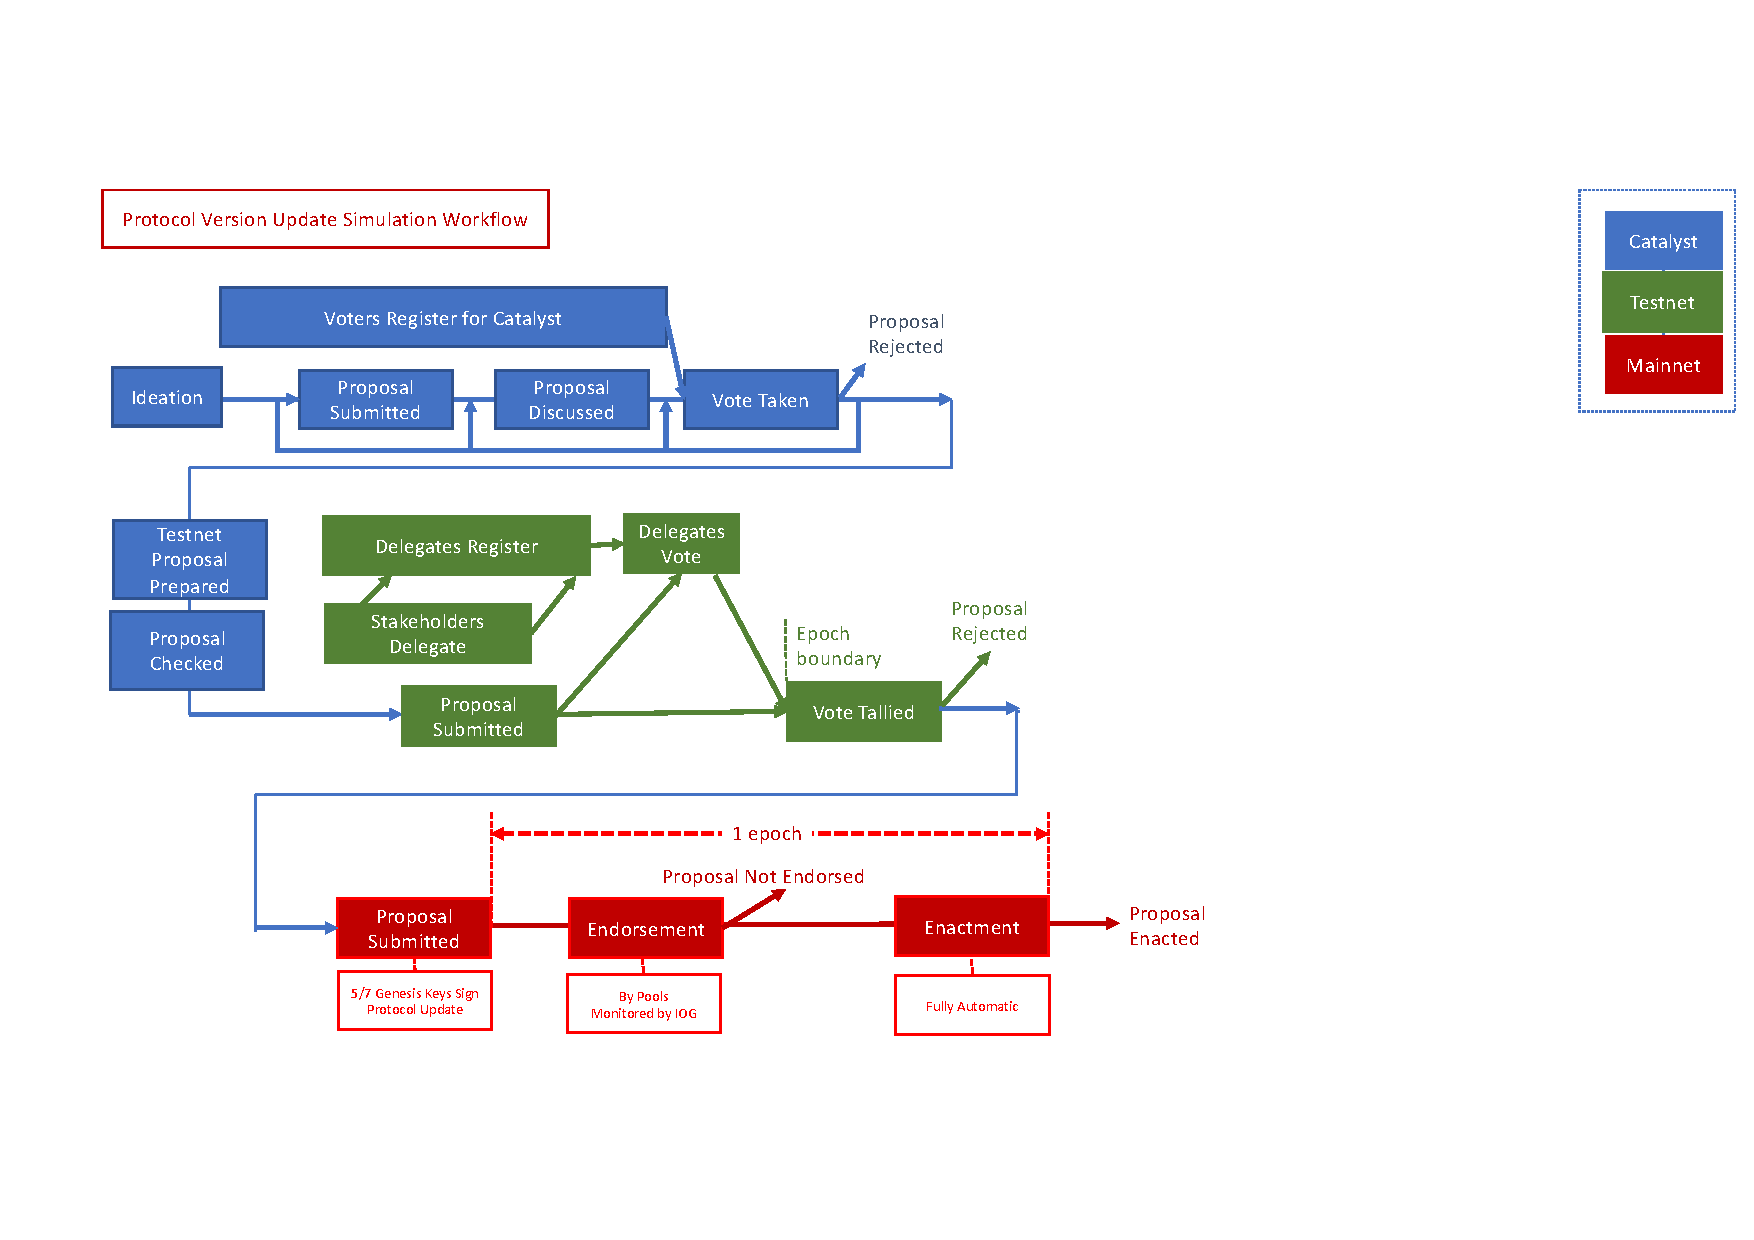
\includegraphics[trim=0 90 0 80,clip,width=\textwidth]{Workflow4}
  \caption{Example Workflow: Protocol Version Update (Hard Fork)}
  \label{fig:workflow-hf}
\end{figure}

\paragraph{Protocol Version Updates (Hard Forks).}  These follow the process described above,
except that the proposal must also be \emph{endorsed} by sufficient stake pool operators
(where endorsement indicates their readiness to upgrade to the new protocol version).
The same process applies to both major and minor protocol version upgrades.
The deadline for endorsement must be given in the original proposal submission.
In order to ensure the stability of the chain, then the endorsement must happen sufficiently before the update takes
effect.  This has been fixed at $XX$ slots prior to the epoch where the proposed is enacted.
If a proposal does not pass the endorsement threshold then it will be rejected at this point, otherwise it will be
passed on for enactment.  It is anticipated that endorsement will be a manual process, though it would be possible
to automate this by monitoring software versions.
While the endorsement deadline will usually be after the voting deadline, this is not technically necessary, and the deadlines could
in principle be contemporaneous, or even reversed.

\paragraph{Rejected Proposals.}  Rejected Proposals are not enacted on-chain.   Once it is rejected, a proposal is never enacted.
An equivalent proposal may, however, be submitted, in which case it must go through the same voting and enactment process
(and may itself be rejected).


\begin{figure}
  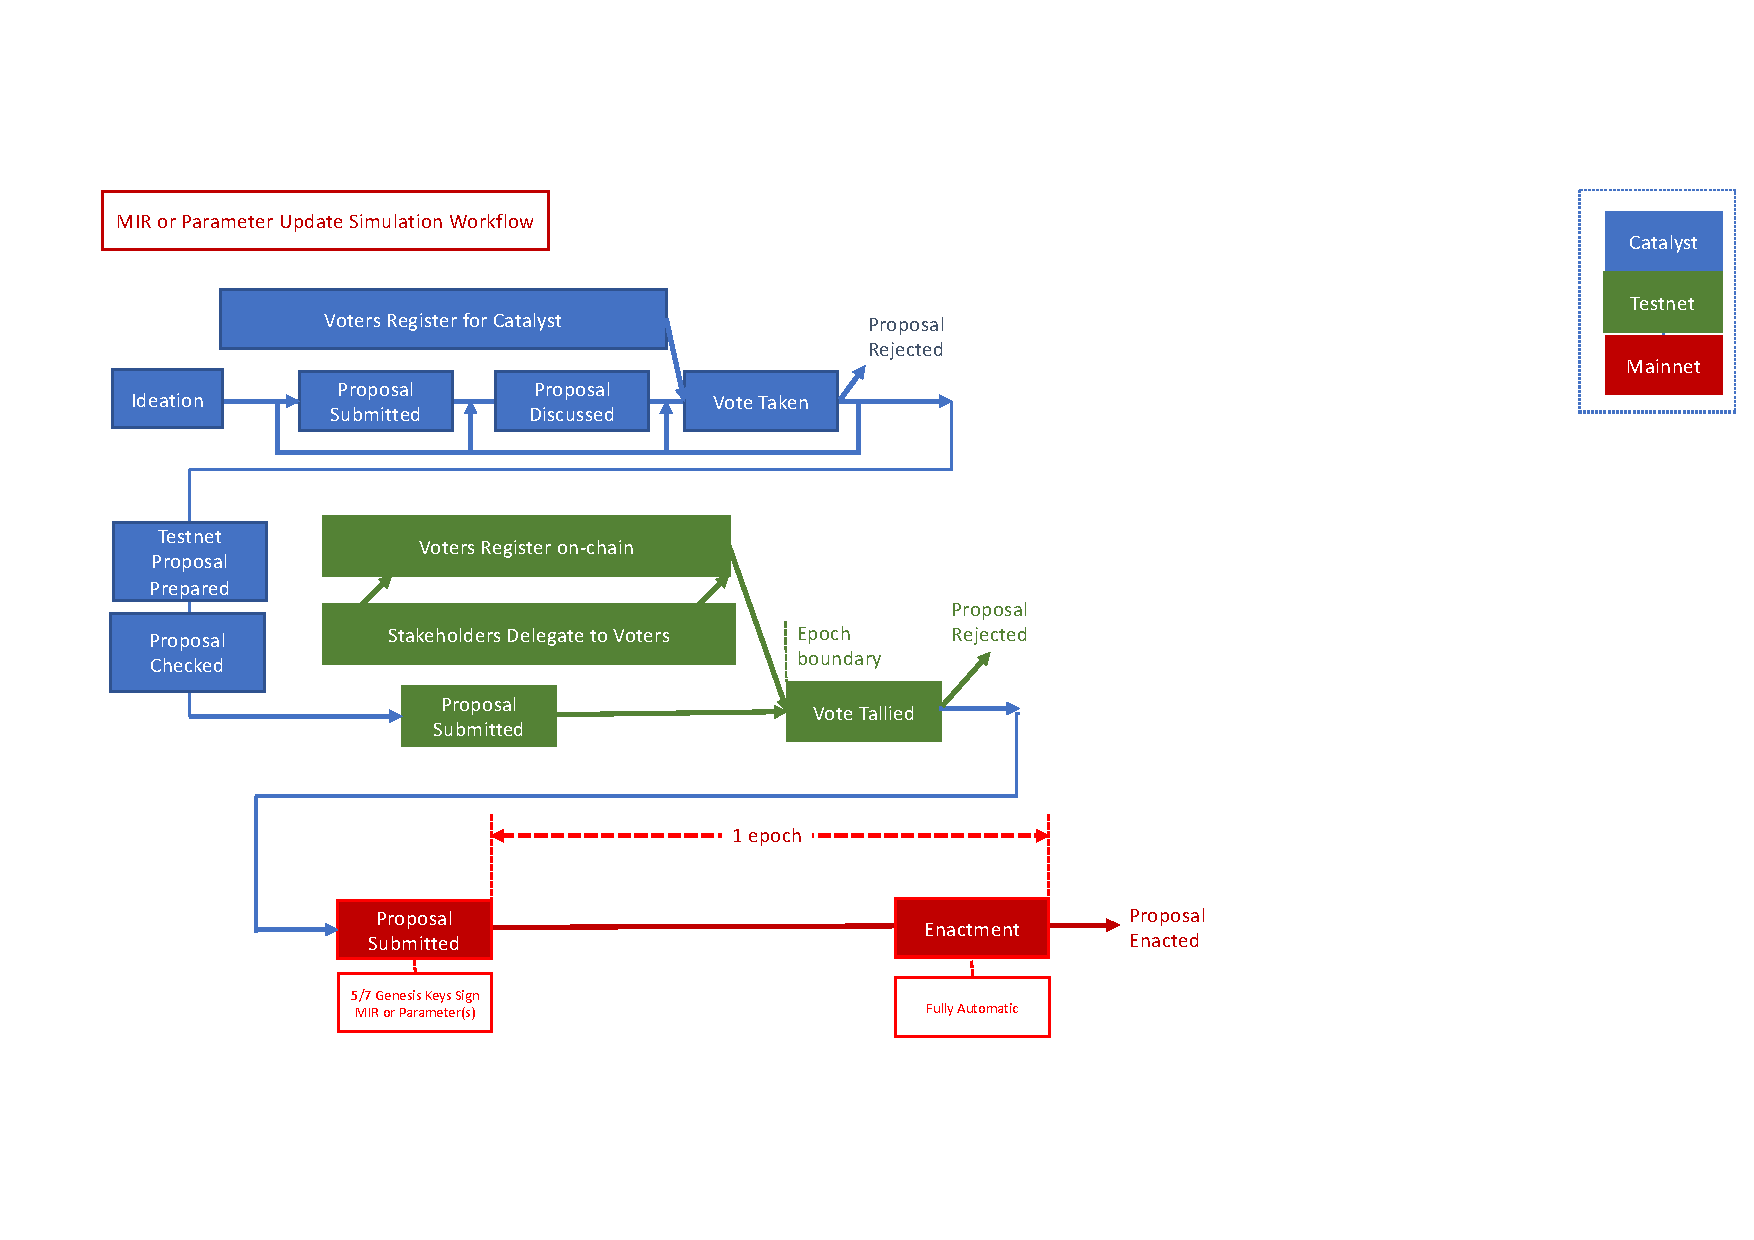
\includegraphics[trim=0 90 0 80,clip,width=\textwidth]{Workflow1}
  \caption{Example Workflow: Funds Transfer (MIR) or Simple Parameter Value Update, showing off-chain delegation and voting simulation steps for initial pilot}
  \label{fig:workflow-mir2}
\end{figure}

\begin{figure}
  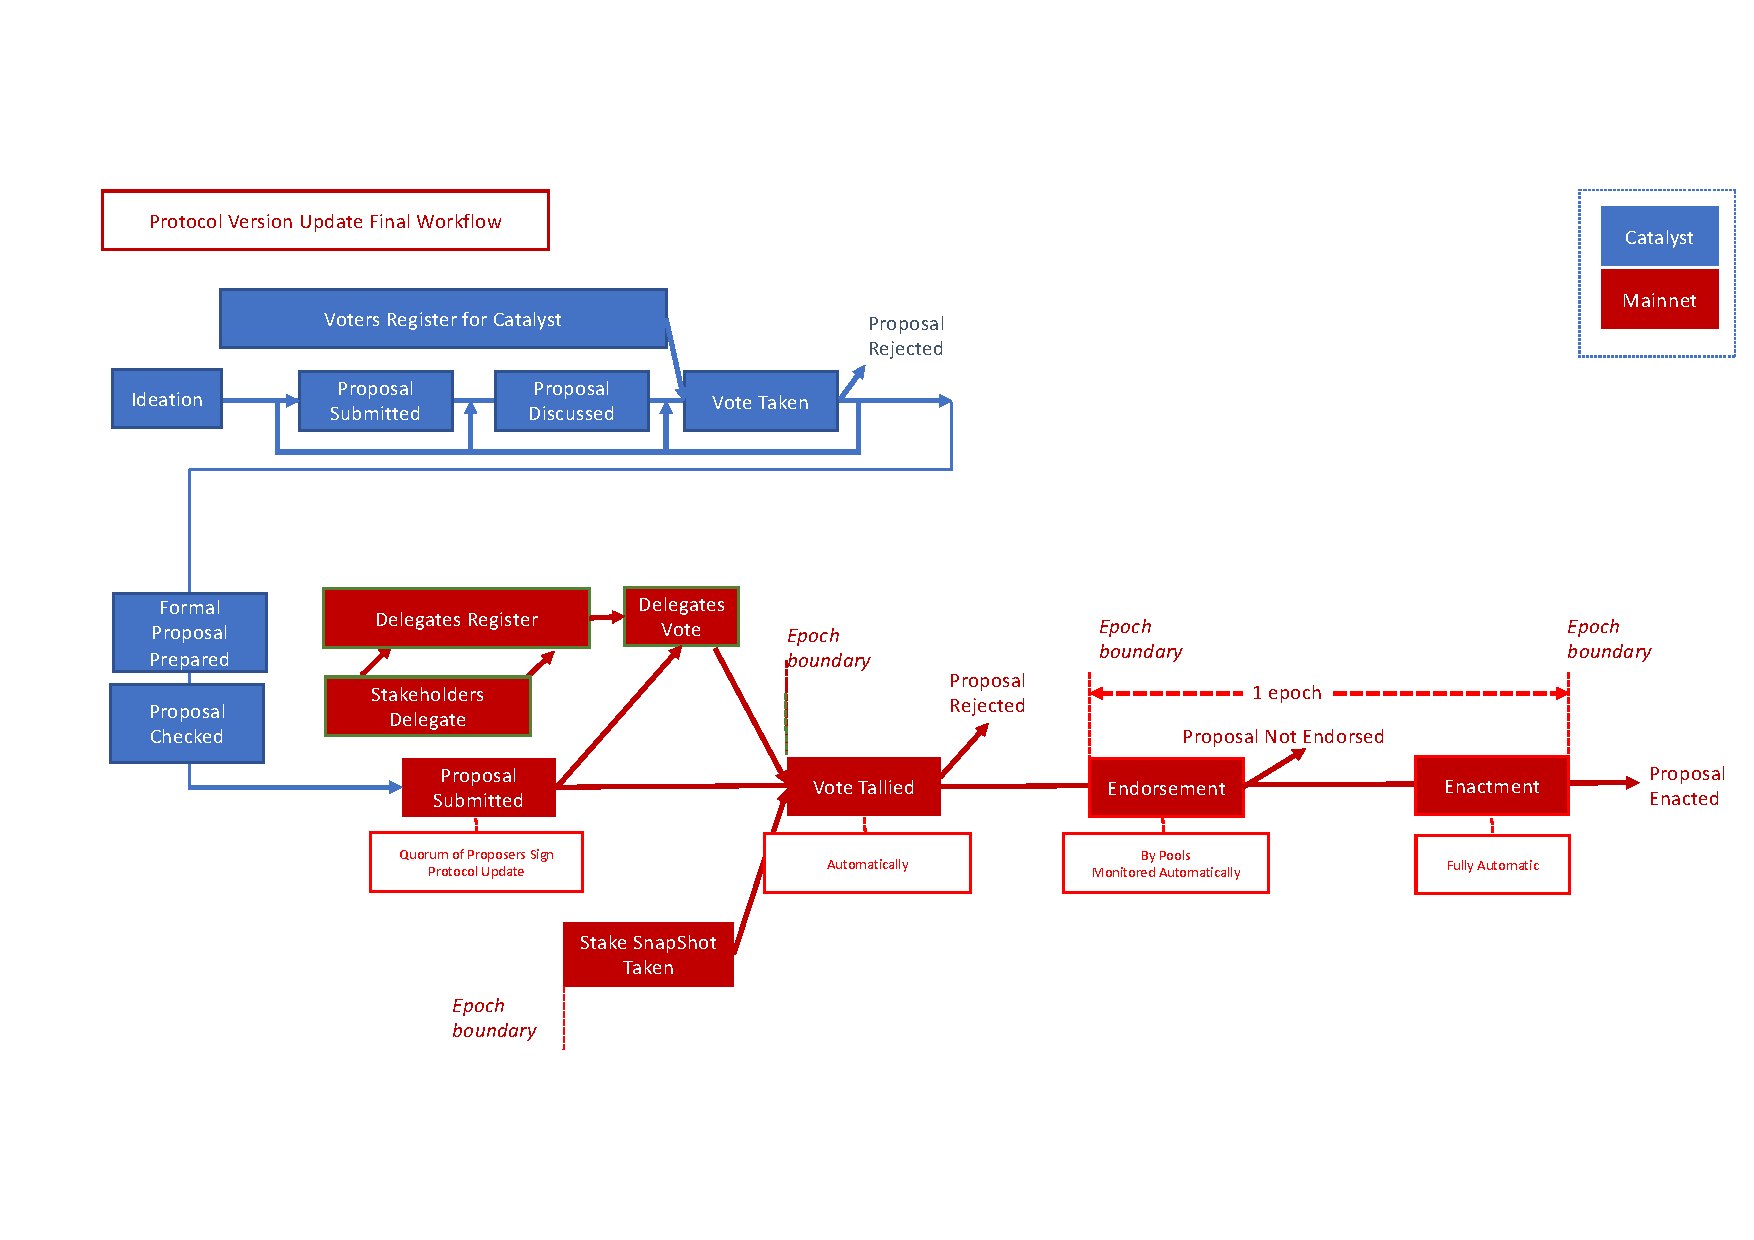
\includegraphics[trim=0 90 0 80,clip,width=\textwidth]{Workflow2}
  \caption{Example Workflow: Protocol Version Update (Hard Fork), showing off-chain delegation and voting simulation steps for initial pilot}
  \label{fig:workflow-hf2}
\end{figure}

\paragraph{Workflows for Accelerating Early Governance Pilots.}

Figures~\ref{fig:workflow-mir2}-\ref{fig:workflow-hf2} show the corresponding  workflows that could be used if desired,
for initial pilots.  The off-chain process is identical in all cases, but the on-chain delegation process is mimicked precisely on a testnet, rather than performed
on-chain.  Accepted proposals are then passed for manual submission and enactment on-chain.  This will allows early testing and tuning of governance mechanisms without
irrevocably changing the on-chain governance process, so permitting more rapid deployment of decentralised governance with reduced implementation and automation risk.

\clearpage
